%%
%% The official i6 slide template _demo_
%% created by Philippe Dreuw and Thomas Deselaers, 2005
%%
%% $Id: slides.tex,v 1.48 2007-11-14 17:13:01 dreuw Exp $
%%
%% Possible options for:
%%  - language       : 'english' (default), 'german'
%%  - page numbering : 'nonumber', 'lastpage' to enable automatic page n/m numbering, 
%%                     'userlastpage' to enable a user defined page n/m numbering using \LastPage command,  
%%                      or leave empty for normal page numbering (default)
%%  - itemize        : 'triangle' or leave empty for bullets (default)
%%  - page titles    : 'allowpagebreaks' to enable titles with automatic page breaks, 
%%                     'nopagebreaks' to disable (default)
%%  - page layout    : 'vertical' to enable vertical centering on each slide using \vfill ... \vfill (default)
%%  - encoding       : 'utf-8' to enable utf encoding instead of latin1 (default)
%%  - tools          : 'blackslide' to insert a black slide which is linked with every slide title, e.g. to write a proof on the blackboard
%%
\documentclass[11pt, a4paper, landscape]{article}
\usepackage{NeyDreuwSlides_Nov07}


%%%%%%%%%%%%%%%%%%%%%%%%%%%%%%%%%%%%%%%%%%%%%%%%%%%%%%%%%%%%%%%%%%%%%%%%%%%%%%%%
%% flyspell can read the local ispelldict variable to automatically change the dictionary, 
%% e.g. german-new8, american, english, british, ...
%% 
%% Local IspellDict: american
%% 


%%%%%%%%%%%%%%%%%%%%%%%%%%%%%%%%%%%%%%%%%%%%%%%%%%%%%%%%%%%%%%%%%%%%%%%%%%%%%%%%
% custom packages
\usepackage{fancyvrb} %%% fancy verbatim to enable coloring within verbatim environments

%\usepackage{pst-node} 

%%%%%%%%%%%%%%%%%%%%%%%%%%%%%%%%%%%%%%%%%%%%%%%%%%%%%%%%%%%%%%%%%%%%%%%%%%%%%%%%
% Some example hacks work only in combination with the 'pdflatex -shell-escape'
% mode. Try 'make hacks'


%%%%%%%%%%%%%%%%%%%%%%%%%%%%%%%%%%%%%%%%%%%%%%%%%%%%%%%%%%%%%%%%%%%%%%%%%%%%%%%%
\renewcommand*{\title}{Graph-Based Image Segmentation}        % main title of the work (used for \TitlePage)
\renewcommand*{\titleshort}{Graph-Based Segmentation}         % short title (used for \lfoot)
\renewcommand*{\occasion}{Seminar medical image processing -- MedBV13}		% (used for \TitlePage)
\renewcommand*{\occasionshort}{MedBV13}               % short occasion title (used for \rfoot)
%\renewcommand*{\date}{11. April 2005}                                        % default is \today (used for \TitlePage and \rfoot)
\renewcommand*{\author}{Phan-Anh Nguyen, Christian Oberdoefer}         % all the authors of the work, can be long (used for \TitlePage)
\renewcommand*{\authorshort}{Phan-Anh et al.:\xspace}                            % all the authors of the work, should be short (used for \lfoot)
\renewcommand*{\email}{\url{anh.nguyen@rwth-aachen.de, oberdoefer@i6.informatik.rwth-aachen.de}}  % all email address(es) of the authors (used for \TitlePage)
\renewcommand*{\mainauthor}{Phan-Anh Nguyen}                                   % the author(s) who presented the work (used for \TitlePage)
\renewcommand*{\mainauthoremail}{\url{anh.nguyen@rwth-aachen.de}}    % presenter mail address(es) (used for \FinalPage)
\renewcommand*{\www}{http://www-i6.informatik.rwth-aachen.de/}                % web address (used for \TitlePage _and_ \FinalPage)
\newcommand*{\keywords}{Graph Cut, Segmentation}                               % keywords, can be used for PDF summary

% will be set into the PDF document summary
\hypersetup{
  pdftitle={\title}, 
  pdfsubject={\occasion},  
  pdfauthor={\author}, 
  pdfkeywords={\keywords},
  % enable automatic page transitions: for endless loop edit in
  % acrobat reader -> preferences -> full screen -> after every X
  % seconds and after last page
  pdfpageduration = 2, 
%  pdfpagetransition = {Glitter /Di 315 /D 5}  
  pdfpagetransition = {Box /M /O /D 1},
}

%%%%%%%%%%%%%%%%%%%%%%%%%%%%%%%%%%%%%%%%%%%%%%%%%%%%%%%%%%%%%%%%%%%%%%%%%%%%%%%%
\listfiles
%%%%%%%%%%%%%%%%%%%%%%%%%%%%%%%%%%%%%%%%%%%%%%%%%%%%%%%%%%%%%%%%%%%%%%%%%%%%%%%%
\begin{document}

%%%%%%%%%%%%%%%%%%%%%%%%%%%%%%%%%%%%%%%%%%%%%%%%%%%%%%%%%%%%%%%%%%%%%%%%%%%%%%%%
\TitlePage

%%%%%%%%%%%%%%%%%%%%%%%%%%%%%%%%%%%%%%%%%%%%%%%%%%%%%%%%%%%%%%%%%%%%%%%%%%%%%%%%
\NewPage\headline{Outline}
\small
\vfill
\begin{enumerate}
\item \hyperlink{sli:introduction}{Introduction - Motivation}
\item \hyperlink{sli:features}{Image Features}
\begin{itemize}
	\item \hyperlink{sli:surf}{Speeded Up Robust Features}
	\item \hyperlink{sli:gPb}{Globalized Probability of Boundary}
\end{itemize}
\item \hyperlink{sli:supervised}{Segmentation with Supervised Learning}
%\begin{itemize}
%	\item \hyperlink{sli:svm}{Support Vector Machine for Region Ranking}
%	\item \hyperlink{sli:logistic}{Logistic Regression}
%	\item \hyperlink{sli:ssm}{Statistical Shape Model}
%\end{itemize}
\item \hyperlink{sli:construction}{Graph Construction}
\begin{itemize}
	\item \hyperlink{sli:region_graph}{Region Graph}
	\item \hyperlink{sli:contour_graph}{Contour Graph}
	\item \hyperlink{sli:mrf}{Markov Random Field}
\end{itemize}
\item \hyperlink{sli:algorithms}{Graph Cut Algorithms}
\begin{itemize}
	\item \hyperlink{sli:PCST}{Prize-Collecting Steiner Tree}
%	\begin{itemize}
%		\item \hyperlink{sli:branch_and_cut}{Branch-and-Cut Algorithm}
%	\end{itemize}
	\item \hyperlink{sli:contour_cut}{Contour Cut}
%	\begin{itemize}
%		\item \hyperlink{sli:circulation}{Graph Circulations}
%		\item \hyperlink{sli:cost}{The Cost Function}
%		\item \hyperlink{sli:solution}{Computational Solution}
%	\end{itemize}
	\item \hyperlink{sli:graph_cut}{Graph-Cut}
%	\begin{itemize}
%		\item \hyperlink{sli:min_cut}{Min-Cut Algorithm}
%		\item \hyperlink{sli:multi_shape}{Multi-Shape Graph-Cuts}
%	\end{itemize}
\end{itemize}
\item \hyperlink{sli:application}{Applications}
%\begin{itemize}
%	\item \hyperlink{sli:ERS}{Efficient Region Search for Object Detection}
%	\item \hyperlink{sli:contour_detector}{Salient Contour Detection}
%	\item \hyperlink{sli:lung_segmentation}{Multi-Shape Graph-Cut for Lung Segmentation}
%\end{itemize}
\item \hyperlink{sli:conclusion}{Conclusion}
\end{enumerate}
%\vfill
%\centerline{\footnotesize PS: the outline should not have more than 5-7 items
%  without any subitems}
%\normalsize
%\vfill


%%%%%%%%%%%%%%%%%%%%%%%%%%%%%%%%%%%%%%%%%%%%%%%%%%%%%%%%%%%%%%%%%%%%%%%%%%%%%%%%
\NewPage\headline{Introduction} 
\hypertarget{sli:introduction}
\vfill
This latex beamer slide style was created by Philippe Dreuw and Thomas
Deselaers and should be used for talks presented at the Lehrstuhl fuer
Informatik 6 at the RWTH Aachen University.
\vfill
Any requests or comments should be sent to
\begin{itemize}
\item \url{mailto:{deselaers,dreuw}@informatik.rwth-aachen.de}
\item \url{http://www-i6.informatik.rwth-aachen.de/}
\end{itemize}
\vfill


%%%%%%%%%%%%%%%%%%%%%%%%%%%%%%%%%%%%%%%%%%%%%%%%%%%%%%%%%%%%%%%%%%%%%%%%%%%%%%%%
\NewPage\headline{Literature} 
\vfill
\begin{itemize}
\item Talks presented at the
  \href{http://www-i6.rwth-aachen.de/}{\isechsicon}
  should always have a literature part in front of the talk. 
\item You should \red{not just copy} bibitems from your \texttt{*.bbl} files
  into a minipage and an \texttt{\textbackslash itemize} environment.
\item Depending on the public where you will present your talk you should adapt
  your literature slide.
\item you should describe the content of the SOTA literature with your
  own words
\end{itemize}
\vfill 

%%%%%%%%%%%%%%%%%%%%%%%%%%%%%%%%%%%%%%%%%%%%%%%%%%%%%%%%%%%%%%%%%%%%%%%%%%%%%%%%
\NewPage\headline{Literature Examples} 
\vfill 
\begin{description}
\item [T.~Starner, J.~Weaver, A.~Pentland:] Real-time american sign-language
  recognition using desk and wearable computer based video. {\em PAMI 1998}.
  \begin{itemize}
  \item HMM based isolated sign language recognition. Explain the main content here.
  \end{itemize}
\item [Povey:] Papertitle. {\em ICASSP 2007}.
  \begin{itemize}
  \item something new in speech recognition. Explain the main content here.
  \end{itemize}
\item \cite{loupias:_wavel_salien_point_image_retriev}: Papertitle. {\em CONFNAME 2007}.
  \begin{itemize}
  \item image retrieval. Explain the main content here.
  \end{itemize}
\end{description}
\vfill


%%%%%%%%%%%%%%%%%%%%%%%%%%%%%%%%%%%%%%%%%%%%%%%%%%%%%%%%%%%%%%%%%%%%%%%%%%%%%%%%
\NewPage\headline{State of the Art} 
\vfill 
\begin{itemize}
\item Talks presented at the
  \href{http:://www-i6.rwth-aachen.de/}{
\includegraphics[height=\baselineskip]{logos/i6-hks44}}
  should also always have a state of the art part in front of the talk.
\item Depending on the public where you will present your talk you should
adapt your state of the art slide.
\item This can be in relation with literature section
\end{itemize}
\vfill

%%%%%%%%%%%%%%%%%%%%%%%%%%%%%%%%%%%%%%%%%%%%%%%%%%%%%%%%%%%%%%%%%%%%%%%%%%%%%%%%
\NewPage\headline{Results} 
\vfill 
\begin{itemize}
\item Talks presented at the
  \href{http:://www-i6.rwth-aachen.de/}{
\includegraphics[height=\baselineskip]{logos/i6-hks44}}
  should always have a result section somewhere at the end of the talk.
\item Depending on the public should highlight the
  advantages/disadvantages of your presented work in comparison to
  other results achieved by other groups on the same (publicly
  available) benchmark database
\end{itemize}
\vfill


%%%%%%%%%%%%%%%%%%%%%%%%%%%%%%%%%%%%%%%%%%%%%%%%%%%%%%%%%%%%%%%%%%%%%%%%%%%%%%%%
%%%%%%%%%%%%%%%%%%%%%%%%%%%%%%%%%%%%%%%%%%%%%%%%%%%%%%%%%%%%%%%%%%%%%%%%%%%%%%%%
\NewPage\headline{The \texttt{HyperSlides} Style}
\hypertarget{sli:style}
\vfill
The following slides will explain how to use the HyperSlides style.
\vfill


%%%%%%%%%%%%%%%%%%%%%%%%%%%%%%%%%%%%%%%%%%%%%%%%%%%%%%%%%%%%%%%%%%%%%%%%%%%%%%%%
\NewPage\headline{Style Parameters}
\vfill
TODO
\vfill


%%%%%%%%%%%%%%%%%%%%%%%%%%%%%%%%%%%%%%%%%%%%%%%%%%%%%%%%%%%%%%%%%%%%%%%%%%%%%%%%
\NewPage\headline{Including Images}
\hypertarget{sli:including_images}
\vfill
\begin{itemize}
\item[] You can include your images with the \\ \texttt{\textbackslash
    includegraphics[options]\{<filename>\}} command. A short caption may be
  written with the \texttt{\textbackslash caption\{<name>\}} command. Examples:
  \begin{figure}
    \centering
    \begin{tabularx}{600pt}{Z Z Z}
      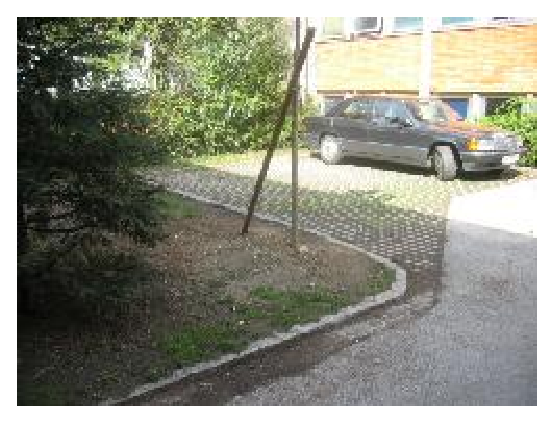
\includegraphics[height=2.5cm]{car}%
      \label{fig:images_car}% 
      \caption{Car}%
      &
      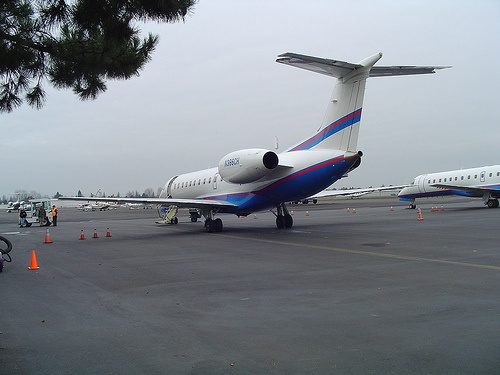
\includegraphics[height=2.5cm]{airplane}%
      \label{fig:images_airplane}% 
      \caption{Airplane}%
      &
      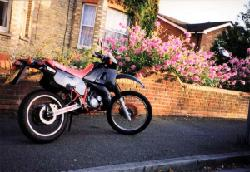
\includegraphics[height=2.5cm]{motorbike}
      \label{fig:images_motorbike}% 
      \caption{Motorbike}%
    \end{tabularx}
    \caption{Images With Caption below}
    \label{fig:images}% 
  \end{figure}
\item[] Images should be scaled relatively to the \texttt{\textbackslash textwidth} or \texttt{\textbackslash linewidth} of the slides:
  \begin{center}
    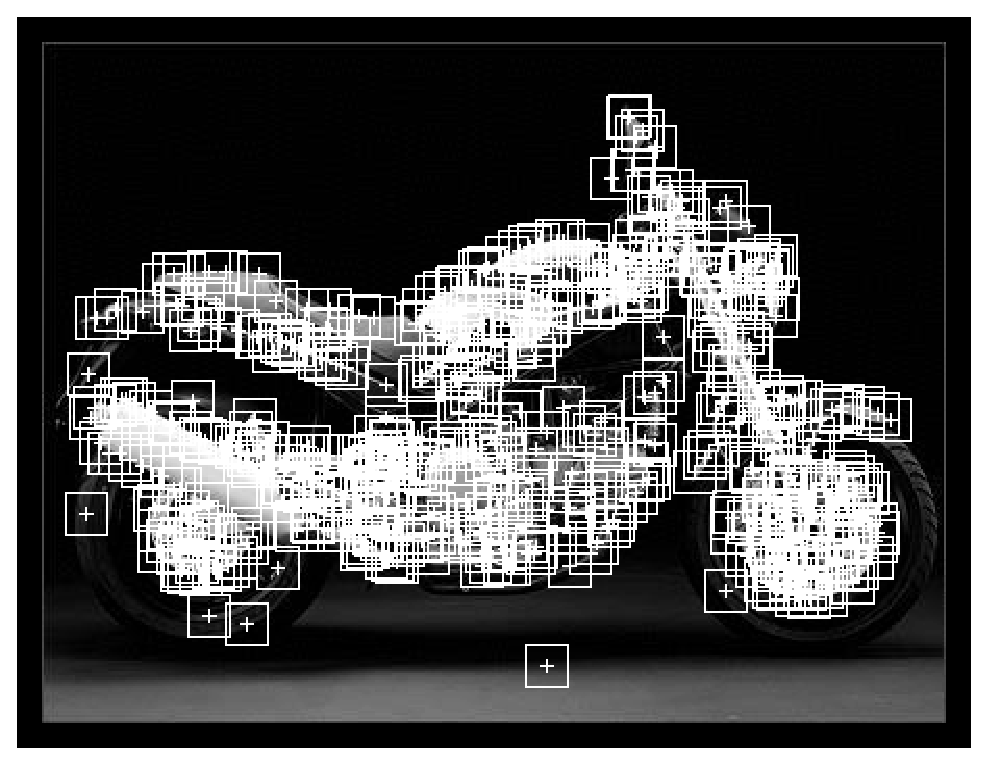
\includegraphics[width=.15\textwidth]{salientpoints}
    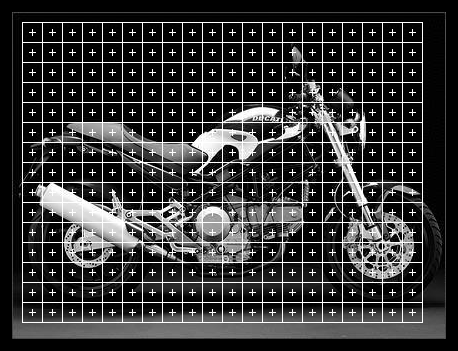
\includegraphics[width=.15\linewidth]{grid}
  \end{center}
\item[] You should always provide images in JPEG/PNG/PDF-- \alert{and}
  EPS/PS--format.
\end{itemize}
\vfill

%%%%%%%%%%%%%%%%%%%%%%%%%%%%%%%%%%%%%%%%%%%%%%%%%%%%%%%%%%%%%%%%%%%%%%%%%%%%%%%%
\NewPage\headline{Including Images}
\vfill
\begin{minipage}[b]{.5\linewidth}
  \begin{center}
    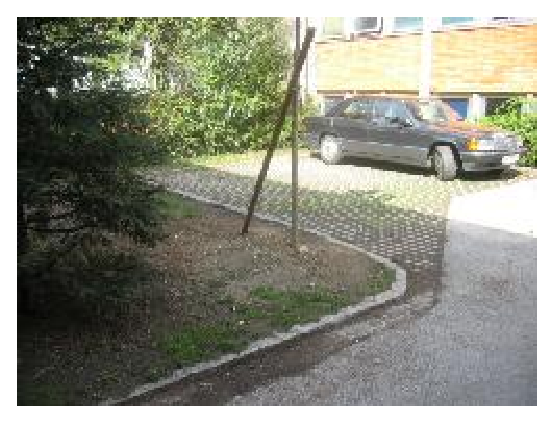
\includegraphics[width=.5\linewidth]{car}\\
    car label
  \end{center}
\end{minipage}
\begin{minipage}[b]{.5\linewidth}
  \begin{itemize}
  \item my
  \item image
  \item description
  \item using \texttt{minipage} environment
  \item my
  \item image
  \item description
  \end{itemize}
\end{minipage}
\vfill

%%%%%%%%%%%%%%%%%%%%%%%%%%%%%%%%%%%%%%%%%%%%%%%%%%%%%%%%%%%%%%%%%%%%%%%%%%%%%%%%
\NewPage\headline{Including Images}
\vfill
\begin{table}
  \centering
  \begin{tabular}{@{} M{.3\linewidth} M{.7\linewidth} @{}}
    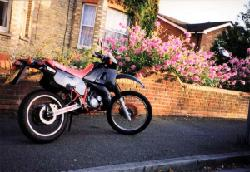
\includegraphics[width=.9\linewidth]{motorbike}
    & 
    \begin{itemize}
    \item my
    \item image
    \item description
    \item using \texttt{tabular} environment
    \item image
    \item description
    \end{itemize}
  \end{tabular}
\end{table}
\vfill

%%%%%%%%%%%%%%%%%%%%%%%%%%%%%%%%%%%%%%%%%%%%%%%%%%%%%%%%%%%%%%%%%%%%%%%%%%%%%%%%
\NewPage\headline{Including Images}
\begin{hvcenter}
  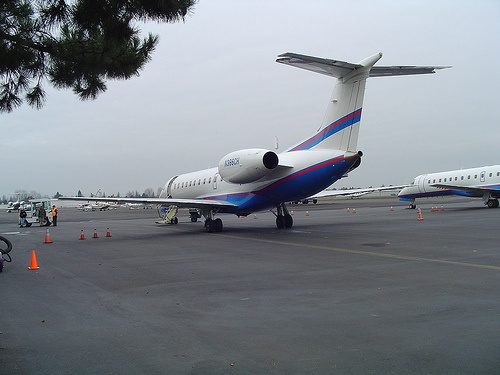
\includegraphics[width=.5\linewidth]{airplane}\\
  my image using \texttt{hvcenter} environment
\end{hvcenter}


%%%%%%%%%%%%%%%%%%%%%%%%%%%%%%%%%%%%%%%%%%%%%%%%%%%%%%%%%%%%%%%%%%%%%%%%%%%%%%%%
\NewPage\headline{Including Images}
\vfill
\begin{itemize}
\item you can insert \texttt{xfig} images in pdftex or pstex manner by \\ using the 
  \texttt{\textbackslash inputfigure\{<filename>\}} \\ or the \texttt{\textbackslash
    inputfigurex\{<filename>\}\{<width>\}\{<height>\}}
\item Example:
  \inputfigure{xfigures/xfigtest} and \inputfigurex{10cm}{1cm}{xfigures/xfigtest}
\item convert the \texttt{xfig}- into \texttt{eps}-images:  
  \texttt{/u/hasan/bin/fig2eps <filename>}
\item if you want to change the image paths, you should redefine the
  \texttt{\textbackslash graphicspath} option and the paths using:
  \begin{footnotesize}
    \begin{itemize}
    \item[] \texttt{\textbackslash renewcommand*\{\textbackslash imagedir\}\{./images/\}}
    \item[] \texttt{\textbackslash renewcommand*\{\textbackslash imagetemplatedir\}\{/u/figures/\}}
    \item[] \texttt{\textbackslash renewcommand*\{\textbackslash xfigdir\}\{./xfigures/\}}
    \item[] \texttt{\textbackslash renewcommand*\{\textbackslash logodir\}\{./logos/\}}
    \item[] \texttt{\textbackslash renewcommand*\{\textbackslash audiodir\}\{./audio/\}}
    \item[] \texttt{\textbackslash renewcommand*\{\textbackslash videodir\}\{./video/\}}
    \item[] \texttt{\textbackslash renewcommand*\{\textbackslash sourcedir\}\{./sources/\}}
    \end{itemize}
  \end{footnotesize}
\item if you want to \alert{extend} the path you should use
  \texttt{\textbackslash extendgraphicspath}
\end{itemize}
\vfill


%%%%%%%%%%%%%%%%%%%%%%%%%%%%%%%%%%%%%%%%%%%%%%%%%%%%%%%%%%%%%%%%%%%%%%%%%%%%%%%%
\NewPage\headline{Including Images}
\vfill
\begin{itemize}
\item free positioning of images or texts using textboxes, look at the z-index
\end{itemize}
\vfill
\begin{textblock}{4}(2,-1) % in runden Klammern die Koordinaten, von der jeweiligen Textstelle aus berechnet
  \scalebox{0.8}{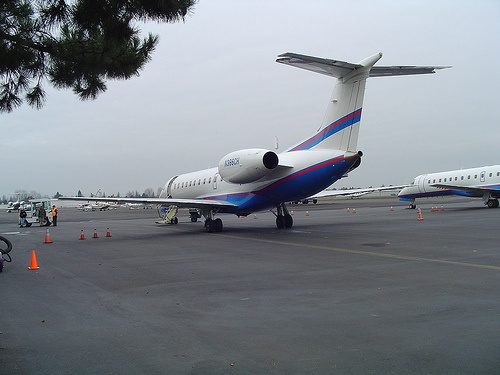
\includegraphics{airplane}}
\end{textblock} 
\begin{itemize}
\item \red{free positioning of images or texts using textboxes}
\end{itemize}
\begin{textblock}{4}(15,-2) % in runden Klammern die Koordinaten, von der jeweiligen Textstelle aus berechnet
  \scalebox{0.8}{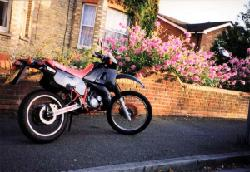
\includegraphics{motorbike}}
\end{textblock} 
\vfill

%%%%%%%%%%%%%%%%%%%%%%%%%%%%%%%%%%%%%%%%%%%%%%%%%%%%%%%%%%%%%%%%%%%%%%%%%%%%%%%%
\NewPage\headline{Default Search Paths}
\hypertarget{sli:search_paths}
\vfill
\begin{itemize}
\item \texttt{<filename>} means the path to the file (with or without parent
  folder depending on the \texttt{\textbackslash graphicspath} option
  \alert{without the file extension} (\eg *.pdf\_t, *.jpg, or *.eps).
\item you can store your \texttt{xfig} figures in the \texttt{./xfigures/}
  folder as this path is already declared in the \texttt{\textbackslash
    graphicspath} option but \texttt{/u/figures} is
  preferred.
\item you can define \texttt{\textbackslash renewcommand*\{\textbackslash
    defaultaudiodir\}\{\textbackslash audiodir\}} to specify the default search
  directory for audio files. [Default is \defaultaudiodir]
\item you can define \texttt{\textbackslash renewcommand*\{\textbackslash
    defaultvideodir\}\{\textbackslash videodir\}} to specify the default search
  directory for video files. [Default is \defaultvideodir]
\item you \alert{should} set \texttt{\textbackslash
    renewcommand*\{\textbackslash defaultaudiodir\}\{\}} \\ or
  \texttt{\textbackslash
    renewcommand*\{\textbackslash defaultvideodir\}\{\}} to clear the default search path for videos in order to use absolute filenames \eg \\
  \texttt{\textbackslash
    videofilelogobox\{/u/wherever/you/want/i6gesture.avi\}}
\end{itemize}
\vfill

%%%%%%%%%%%%%%%%%%%%%%%%%%%%%%%%%%%%%%%%%%%%%%%%%%%%%%%%%%%%%%%%%%%%%%%%%%%%%%%%
\NewPage\headline{Including Images: Recommendation}
\vfill
\begin{itemize}
\item \red{You should always specify the full image path for images from \\
    \texttt{/u/figures/<user>/<name>\_<User>\_<DDMmmYY>}} \\
  \eg \texttt{/u/figures/dreuw/TangentDistance\_Dreuw\_18Jul06}
\item \red{do not use} the package \texttt{epsf} or \texttt{psfig} (\ra replaced by \texttt{graphicx.sty})
  %\item \texttt{epsf} is only a wrapper for \texttt{graphicx} for old documents
  % created using \texttt{psfig}
\item you can use \texttt{\textbackslash usepackage\{afterpage\}} to flush all
  images first before the next text part begins, by calling
  \texttt{\textbackslash afterpage\{\textbackslash clearpage\}}
\item do \red{not use the following deprecated commands}, as they will cause
  problems with pdfTeX (pdfTeX can also run in DVI-mode).
\begin{verbatim}
\newif\ifpdf
\ifx\pdfoutput\undefined
    \pdffalse       %NO Pdflatex
\else
    \pdfoutput=1    %PDFLatex
    \pdftrue
\fi 
\end{verbatim}
\item \alert{\texttt{\textbackslash usepackage\{ifpdf\}}} is already part of the
  style and runs also under \hyphenation{MacOSX} MacOSX and is used instead. It
  provides the \texttt{\textbackslash ifpdf} command.
\end{itemize}
\vfill

%%%%%%%%%%%%%%%%%%%%%%%%%%%%%%%%%%%%%%%%%%%%%%%%%%%%%%%%%%%%%%%%%%%%%%%%%%%%%%%%
\NewPage\headline{Running External Applications}
\hypertarget{sli:hyperlinks_external}
\vfill
\begin{itemize}
\item You can call every external application with \texttt{\textbackslash
    href\{run:<script>\}} command.  For this you have to specify a shell
  script, in which you can execute any system commands. This will work with Xpdf
  \href{http://www.foolabs.com/xpdf/}{
\includegraphics[scale=0.5]{logos/xpdf}}
  \alert{and} AdobeAcrobat
  \href{http://www.adobe.com/products/acrobat/readstep2.html}{
\includegraphics[scale=0.5]{logos/acrobat}}.
\item \href{run:scripts/demo.sh}{Shell demo starting xclock} will open a new
  terminal which will start the \texttt{xclock} on your computer.
\item Also you can use this command to play movies. Clicking on the image will
  play a movie
  \href{run:\videodir/lti.mpg}{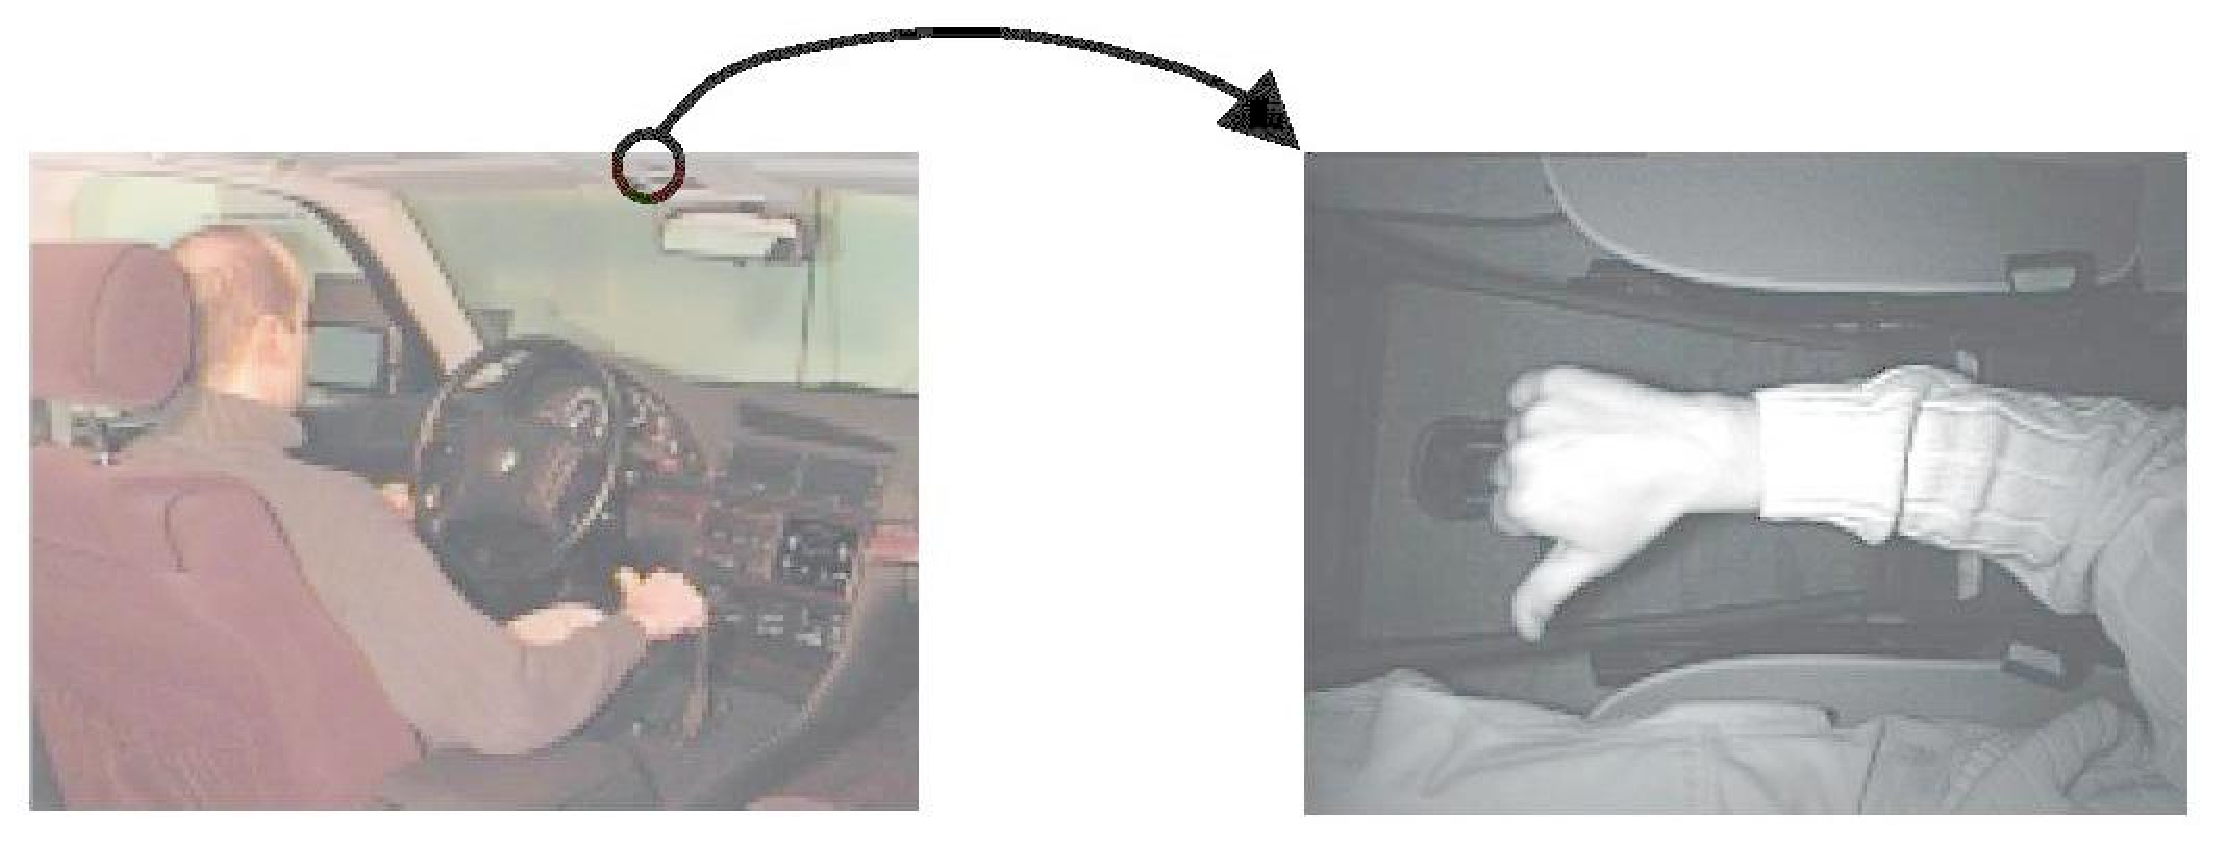
\includegraphics[scale=0.15]{\videodir/lti}}
\end{itemize}
\vfill

%%%%%%%%%%%%%%%%%%%%%%%%%%%%%%%%%%%%%%%%%%%%%%%%%%%%%%%%%%%%%%%%%%%%%%%%%%%%%%%%
\NewPage\headline{Hyperlinks}
\vfill
\begin{itemize}
\item You can link to an url with the \texttt{\textbackslash url\{<link>\}}
  command, \eg \url{www.google.com}. If you have a long url name or you want
  to change the name of the url anchor then use \texttt{\textbackslash
    href\{<link>\}\{<name>\}}, \eg \href{http://www.google.com}{Google}.
\item use the \texttt{\textbackslash urllogo\{<link>\}} or
  \texttt{\textbackslash urllogobox\{<link>\}} to create links with an
  additional icon before like \urllogo{www.google.com} or
  \urllogobox{www.google.com}
\item With the \texttt{\textbackslash hyperlink\{<anchor>\}\{<linkname>\}} and \\
  \texttt{\textbackslash hypertarget\{<anchor>\}\{<targetname>\}} commands you
  can create links inside your slides.  Example: this can be usefull to
  \hyperlink{anchorname}{link to slides from the appendix} (\eg the data used
  to create a plot).
\item Use the \texttt{\textbackslash autoref\{<anchor>\}} command to
  automatically refer to \autoref{fig:images}, \autoref{eq:histogram_formula},
  or \autoref{tab:table}.
\end{itemize}
\vfill


%%%%%%%%%%%%%%%%%%%%%%%%%%%%%%%%%%%%%%%%%%%%%%%%%%%%%%%%%%%%%%%%%%%%%%%%%%%%%%%%
\NewPage\headline{Playing Audio Files}
\hypertarget{sli:hyperlinks_audio}
\vfill
Audio examples from the Verbmobil corpus:
\begin{footnotesize}
  \begin{itemize}
  \item \texttt{\textbackslash audiofilelogobox\{<file>\}}:
    \audiofilelogobox{example-verbmobil-1.wav}
  \item \texttt{\textbackslash audiofilelogo\{<file>\}}:
    \audiofilelogo{example-verbmobil-3.wav}
  \item \texttt{\textbackslash audiofilebox\{<file>\}}:
    \audiofilebox{example-verbmobil-2.wav}
  \item \texttt{\textbackslash audiofile\{<file>\}}:
    \audiofile{example-verbmobil-1.wav}
  \item \texttt{\textbackslash audiofiletext\{<file>\}\{<text>\}}:
    \audiofiletext{example-verbmobil-2.wav}{Example 2 from Verbmobil2}
  \end{itemize}
\end{footnotesize}
\vfill

%%%%%%%%%%%%%%%%%%%%%%%%%%%%%%%%%%%%%%%%%%%%%%%%%%%%%%%%%%%%%%%%%%%%%%%%%%%%%%%%
\NewPage\headline{Playing Video Files}
\hypertarget{sli:hyperlinks_video}
\vfill
%
%\renewcommand*{\defaultvideodir}{} 
% -> if set, you could write \eg \videofilelogobox{/u/wherever/you/want/i6gesture.avi} 
%    or \videofilelogobox{./video/i6gesture.avi} instead of only \videofilelogobox{i6gesture.avi}
%
\renewcommand*{\defaultvideodir}{}
Video examples from the LTI--Gesture and i6--Gesture database:
\begin{footnotesize}
  \begin{itemize}
  \item \texttt{\textbackslash
      videofilethumbnailbox\{<file>\}\{<param>\}\{<image>\}}:
    \videofilethumbnailbox{\videodir/lti.mpg}{scale=0.1}{\videodir/lti}
  \item \texttt{\textbackslash
      videofilethumbnail\{<file>\}\{<param>\}\{<image>\}}:
    \videofilethumbnail{\videodir/lti.mpg}{scale=0.1}{\videodir/lti} %use scale=1.0 to disable scaling
  \item \texttt{\textbackslash videofilelogobox\{<file>\}}:
    \videofilelogobox{\videodir/i6gesture.avi}
  \item \texttt{\textbackslash videofilelogo\{<file>\}}:
    \videofilelogo{\videodir/i6gesture.avi}
  \item \texttt{\textbackslash videofilebox\{<file>\}}: \videofilebox{\videodir/i6gesture.avi}
  \item \texttt{\textbackslash videofile\{<file>\}}: \videofile{\videodir/i6gesture.avi}
  \item \texttt{\textbackslash videologo\{<file>\}}: \videologo{\videodir/i6gesture.avi}
  \item \texttt{\textbackslash videofiletext\{<file>\}\{<text>\}}:
    \videofiletext{./video/i6gesture.avi}{Example from i6--Gesture database} %here with absolute/relative path!
  \end{itemize}
\end{footnotesize}
\vfill 
There are also icons for CDs \cdicon and DVDs \dvdicon which you can use to play
videos from an external device. Just write a script to mount the device and a
player command which will start playing a file from the mounted device.
\vfill


%%%%%%%%%%%%%%%%%%%%%%%%%%%%%%%%%%%%%%%%%%%%%%%%%%%%%%%%%%%%%%%%%%%%%%%%%%%%%%%%
%%%%%%%%%%%%%%%%%%%%%%%%%%%%%%%%%%%%%%%%%%%%%%%%%%%%%%%%%%%%%%%%%%%%%%%%%%%%%%%%
\NewPage\headline{\LaTeX \ Tips} 
\vfill
Some general \LaTeX \ recommendations and tips
\begin{itemize}
\item replace: \texttt{\$\$...\$\$} by
  \texttt{\textbackslash[...\textbackslash]}
\item replace: \texttt{\textbackslash centerline\{...\}} by
  \texttt{\{\textbackslash centering ...\}} or the \texttt{center}
  environment
\item replace: \texttt{eqnarray} environment where possible by \texttt{align}
\end{itemize}
\vfill

%%%%%%%%%%%%%%%%%%%%%%%%%%%%%%%%%%%%%%%%%%%%%%%%%%%%%%%%%%%%%%%%%%%%%%%%%%%%%%%%
\NewPage\headline{Formulas} 
\hypertarget{sli:formulas} 
\vfill 
Write formulas with the \texttt{\textbackslash begin\{equation\}} environment or
with the double \texttt{\$\$} signs, use a single \texttt{\$} sign if you want
to write a formula on the same text line.  
\vfill
\begin{itemize}
\item numbered equation 
  \begin{equation}
    h_c(X) = \frac{1}{L_X} \sum_{l=1}^{L_X} \delta(c,c(x_l)) \label{eq:histogram_formula}
  \end{equation}
\item unnumbered equation 
  \begin{equation}
    h_c(X) = \frac{1}{L_X} \sum_{l=1}^{L_X} \delta(c,c(x_l)) \nonumber
  \end{equation}
  or use 
  \[ h_c(X) = \frac{1}{L_X} \sum_{l=1}^{L_X} \delta(c,c(x_l)) \] %%  i.e. do not use '$$...$$' which is deprecated
\item with $ h_c(X) = \frac{1}{L_X} \sum_{l=1}^{L_X}
  \delta(c,c(x_l))$ on the same line.  
\end{itemize}
%  with 
%    \begin{center}
%      \begin{tabular}{ll}
%        $L_X$ & number of patches for image $X$\\
%        $x_l$ & $l$-th patch for image $X$\\
%        $c(x_l)$ & closest cluster identifier for $x_l$\\
%        $h_c(X)$ & $c$-th bin of histogram for image $X$\\
%      \end{tabular}
%    \end{center}
\vfill

%%%%%%%%%%%%%%%%%%%%%%%%%%%%%%%%%%%%%%%%%%%%%%%%%%%%%%%%%%%%%%%%%%%%%%%%%%%%%%%%
\NewPage\headline{Tables} 
\hypertarget{sli:tables} 
\vfill 
You can use the \texttt{\textbackslash begin\{table\}} environment to present
your results. Also you can link the whole table to another slide with the
\texttt{\textbackslash hyperlink} command in combination with
\texttt{\textbackslash textcolor\{black\}}, otherwise the table would appear in
link color.
\vfill
Some results achieved at the \isechsicon.
\begin{table}
  \centering
  \caption{Table caption above. \alert{Click on the table} to jump to the \appendixname}
  \hyperlink{table_data}{\textcolor{black}{%
      \begin{tabular}{|l|l|l|l|l|}
        \hline
                              &  motorbikes   &   bicycles &   people   & cars     \\
        \hline
        Task 1                &  6,8 (17)     &  5,8 (15)  & 5,6 (15)   & 4,5 (17) \\
        Task 2&  2,3 (11)     &  2,3 (9)      & 2,3 (9)    & 2,3 (10)              \\
        \hline
      \end{tabular}
    }
  }
  \label{tab:table}
\end{table}
\vfill

%%%%%%%%%%%%%%%%%%%%%%%%%%%%%%%%%%%%%%%%%%%%%%%%%%%%%%%%%%%%%%%%%%%%%%%%%%%%%%%%
\NewPage\headline{Tables} 
\vfill
\begin{table}      
  %\footnotesize
  \centering
  \caption{Error rates [\%] using the nicer \emph{booktabs style} ordered by decimal position}
  \begin{tabular}{@{} l D{2.4} D{10.10} D{2.2} @{}}
    \toprule  
    \multicolumn{1}{@{}N}{Spatial derivative} & \multicolumn{1}{N}{Original} & \multicolumn{1}{N}{1st time derivative} & \multicolumn{1}{N@{}}{2nd time derivative} \\ 
    \multicolumn{1}{@{}N}{(Sobel)}  &                            &                            &                                                     \\ 
    \midrule      
    
    no                              &  0.0001                    &  0.0001                      & 15.7                                                \\
    horizontal                      &  0.001                     &  0.001                       & 20.0                                                \\
    vertical                        &  1.01                      &  1.01                        & 16.4                                                \\ 
    magnitude                       & 10                         & 10                           &  7.1                                                \\ 
    squared magnitude               & 11.1                       & 11.1                         & 34.2                                                \\ 
    \bottomrule
  \end{tabular}
  \label{tab:table_book}
\end{table}
\vfill
\begin{table}      
  %\footnotesize
  \centering
  \caption{Table using cmidrule command and rotated column heads}
  \begin{tabular}{@{} l l D{2.2} D{2.2} @{}}
    \toprule 
    \multicolumn{1}{@{}N}{Densities}  & \multicolumn{1}{S{5em}}{\alert{Pooling}}  & \multicolumn{1}{t{5em}}{\alert{Gaussian ER[\%]}} & \multicolumn{1}{R{5em}@{}}{Laplacian ER[\%]} \\ 
    \cmidrule(r){1-1}                   \cmidrule(lr){2-2}                          \cmidrule(lr){3-3}                                 \cmidrule(l){4-4} 
    Single                            & No                                        & 29.2                                             & 30.7                                         \\
                                      & Yes                                       & 29.2                                             & 30.7                                         \\ 
    \addlinespace                                                                                                                  
    Mixture                           & No                                        & 21.4                                             & 29.2                                         \\ 
                                      & Yes                                       & 23.5                                             & 27.8                                         \\ 
    \bottomrule
  \end{tabular}
  \label{tab:basic-hmm-difference-0-1}
\end{table}
\vfill
\begin{table}      
  \centering
  \caption{Table using cmidrule command and rotated column heads}
  \begin{tabular}{@{} l M{7cm} V{3cm} D{2.2} c @{}}
    \toprule 
    Type & \multicolumn{2}{c}{Features} & \multicolumn{1}{N}{Error Rate} & \multicolumn{1}{V{5cm}@{}}{Info}\\
    \cmidrule(lr){2-3}
    &
    \multicolumn{1}{R{6em}}{Long Feature description 1} 
    &
    \multicolumn{1}{R{6em}}{Long Feature description 2} 
    &
    &
    \\
    \cmidrule(r){1-1}\cmidrule(lr){2-2}\cmidrule(lr){3-3}\cmidrule(lr){4-4}\cmidrule(l){5-5}
    nice 
    & 
    feature very long and centered baseline with fixed width feature very long and centered baseline 
    with fixed width feature very long and centered baseline  with fixed width 
    & description very long and NOT centered with fixed width 
    & 1.23\% 
    & horizontal centered w/o width\\
    \bottomrule
  \end{tabular}
  \label{tab:cmidrule-rotated-vcentered}
\end{table}    
\vfill
\begin{table}      
  \centering
  \caption{Table using *-command}
  \begin{tabular}{@{} *{4}{l} @{}}
    \toprule 
    \multicolumn{1}{@{}n}{Nominativ} & \multicolumn{1}{n}{Genetiv}    & \multicolumn{1}{n}{Dativ}     & \multicolumn{1}{@{}n}{Akkusativ} \\
    \midrule
    die Frau  & der Frau   & der Frau  & die Frau  \\
    der Mann  & des Mannes & dem Manne & den Mann  \\
    das Kind  & des Kindes & dem Kinde & das Kind  \\
    \bottomrule
  \end{tabular}
\end{table}
\vfill

%%%%%%%%%%%%%%%%%%%%%%%%%%%%%%%%%%%%%%%%%%%%%%%%%%%%%%%%%%%%%%%%%%%%%%%%%%%%%%%%
\NewPage\headline{Citing} 
\hypertarget{sli:citing} 
\vfill 
Use the \texttt{\textbackslash cite\{<anchor>\}}
command to refer to an entry in your bibliography. You can click on the citation
to jump to your bibliography. 

You can use the backreferences in the bibliography to jump back to your slide.
\vfill
\begin{enumerate}[{Example*} a)]
\item Results on Caltech database:
  \cite{deselaers05:_discr_train_objec_recog_image_patch}\\
  very good on motorbikes and airplanes, quite good on faces
  \vfill
\item Results on medical
  radiographs:\cite{loupias:_wavel_salien_point_image_retriev}\\
  quite good, specialized approaches are better
  \vfill
\end{enumerate}
\vfill
Use the package \texttt{\textbackslash usepackage\{cite\}} to sort your cites
\vfill 
{\footnotesize *The enumerate environment from the \texttt{paralist} package can use
  special labels.}  
\vfill


%%%%%%%%%%%%%%%%%%%%%%%%%%%%%%%%%%%%%%%%%%%%%%%%%%%%%%%%%%%%%%%%%%%%%%%%%%%%%%%%
\NewPage\headline{\textcolor{red}{C}\textcolor{green}{o}\textcolor{blue}{l}\textcolor{red}{o}\textcolor{green}{r}\textcolor{blue}{s}}
\hypertarget{sli:colors}
\vfill
\begin{itemize}
  \setlength\itemsep{2ex}   %%% redefines itemsep only for this section
\item How to \alert{highlight} words? This can be done by the
  \texttt{\textbackslash alert\{<text>\}} command. You should use this command
  for \alert{important} words.
\item You can use \textcolor{red}{additional} \textcolor{green}{colors} with the
  \texttt{\textbackslash textcolor\{<color>\}} \magenta{command} in your
  \blue{slides} to \red{highlight} \green{words}, but don't use \magenta{too}
  \isechsbluedark{much} \isechsblue{colors}! \\ The \texttt{\textbackslash
    alert\{<text>\}} command should always be \alert{preferred}
\end{itemize}
\vfill
Spoken:
\begin{quote}
  also ich vielleicht ist grade zu der Zeit die CeBit das w\"are
  vielleicht f\"ur uns fachlich auch ganz interessant
\end{quote}
Recognized:
\begin{quote}
  also ich vielleicht \textcolor{red}{das} grade zu der Zeit die
  CeBit das w\"are vielleicht \textcolor{red}{---} uns fachlich auch
  \textcolor{green}{noch} ganz interessant
\end{quote}
\textcolor{red}{substitution}
\qquad
\textcolor{green}{insertion}
\qquad
\textcolor{red}{---} deletion
\vfill
\begin{equation*}
  \textrm{WER} =
  \frac{1 \textrm{ deletion} + 1\textrm{ insertion} + 1\textrm{ substitution}}
  {19 \textrm{ spoken words}} = 15.8 \%
\end{equation*}
\vfill


%%%%%%%%%%%%%%%%%%%%%%%%%%%%%%%%%%%%%%%%%%%%%%%%%%%%%%%%%%%%%%%%%%%%%%%%%%%%%%%%
\NewPage\headline{Page Numbering}
\hypertarget{sli:pagenumbering}
\vfill
\begin{itemize}
\item you can use the package option \texttt{lastpage} or \texttt{userlastpage}
  to enable a page numbering like ``n of m'', otherwise the pages will have a
  single page number.
\item if you use the package option \texttt{userlastpage} \alert{you have to} call
  \texttt{\textbackslash LastPage} \\ or \texttt{\textbackslash FinalPage} at the
  end of your last slide to enable a correct numbering of the slides.
\item \texttt{\textbackslash FinalPage} will automatically generate a ``Thank
  you for your attention page'' with your name, email and www address.
\item you can change the layout of \emph{your} last page by using
  \texttt{\textbackslash LastPage} at the end of your last slide. This will
  simply insert a blank page and enable a correct numbering of the
  slides.
\item you can also use \texttt{\textbackslash LastPage} or
  \texttt{\textbackslash FinalPage} without specifying the package option
  \texttt{lastpage}. This won't affect the page numbering.
\item to disable the page numbering you must use the the package option
  \texttt{nonumber}.
\end{itemize}
\vfill

%%%%%%%%%%%%%%%%%%%%%%%%%%%%%%%%%%%%%%%%%%%%%%%%%%%%%%%%%%%%%%%%%%%%%%%%%%%%%%%%
\NewPage\headline{Changing Logos}
\hypertarget{sli:logos}
\vfill
\renewcommand*{\topleftlogo}{\includegraphics[height=10mm, width=2cm]{\logodir TT2logo}}
\begin{itemize}
\item you can display a third logo in the topleft corner on each slide by redefining 
  \texttt{\textbackslash topleftlogo}
  \begin{itemize}
  \item Example 1: \newline \footnotesize{\texttt{\textbackslash renewcommand*\{\textbackslash topleftlogo\}\{\textbackslash includegraphics[height=6mm]\{\textbackslash logodir YOUR--THIRD-LOGO\}\} }} \normalsize
  \item Example 2: \newline \footnotesize{\texttt{\textbackslash renewcommand*\{\textbackslash topleftlogo\}\{\textbackslash includegraphics[height=6mm]\{/u/path/to/your/third/LOGO\}\} }} \normalsize
  \end{itemize}
\item Also you could redefine the other logos \texttt{\textbackslash
    toprightlogo} \newline and \texttt{\textbackslash bottomrightlogo} in this way
\item if you are still not happy you might change \texttt{\textbackslash lhead},
  \texttt{\textbackslash rhead} or \texttt{\textbackslash rfoot} at your own
  ``risk''
\end{itemize}
\vfill

%%%%%%%%%%%%%%%%%%%%%%%%%%%%%%%%%%%%%%%%%%%%%%%%%%%%%%%%%%%%%%%%%%%%%%%%%%%%%%%%
\NewPage\headline{Page Titles} \renewcommand*{\topleftlogo}{} %% remove the third logo defined at the previous slide
\hypertarget{sli:titles} 
\vfill 
You can break pages if you choose the option \texttt{allowpagebreaks}, the title
will be repeated on the next slide ...  
\vfill 
\NewPage
\vfill 
... as you can see (or not, depending on the option) !  
\vfill

%%%%%%%%%%%%%%%%%%%%%%%%%%%%%%%%%%%%%%%%%%%%%%%%%%%%%%%%%%%%%%%%%%%%%%%%%%%%%%%%
\NewPage\headline{Overlay Slides}
\vfill
\begin{itemize}
\item you can use the \texttt{\textbackslash NewOverlay} command to create
  overlay slides, i.e.\ to correctly number the pages
\item you will get pdfTeX warnings about duplicate identifiers with
  \texttt{pdflatex}. Use \texttt{make slides.pdf} instead.
  \begin{itemize}
  \item \textcolor{gray}{not yet ...}  % or use white instead of gray
  \end{itemize}
\end{itemize}
\vfill

%%%%%%%%%%%%%%%%%%%%%%%%%%%%%%%%%%%%%%%%%%%%%%%%%%%%%%%%%%%%%%%%%%%%%%%%%%%%%%%%
\NewOverlay\headline{Overlay Slides}
\vfill
\begin{itemize}
\item you can use the \texttt{\textbackslash NewOverlay} command to create
  overlay slides, i.e.\ to correctly number the pages
\item you will get pdfTeX warnings about duplicate identifiers with
  \texttt{pdflatex}. Use \texttt{make slides.pdf} instead.
  \begin{itemize}
  \item not yet ... but now, and look at the page number
  \end{itemize}
\end{itemize}
\vfill

%  %%%%%%%%%%%%%%%%%%%%%%%%%%%%%%%%%%%%%%%%%%%%%%%%%%%%%%%%%%%%%%%%%%%%%%%%%%%%%%%%
%  \NewCenteredPage\headline{Centered Slides}
%  \begin{itemize}
%  \item you can use the \texttt{\textbackslash NewOverlay} command to create vertical centered slides
%  \item this may cause problems when you change between normal and automatically
%    centered slides!
%  \end{itemize}
%  \vfill % because we use only one \NewCenteredPage command here ... 

%%%%%%%%%%%%%%%%%%%%%%%%%%%%%%%%%%%%%%%%%%%%%%%%%%%%%%%%%%%%%%%%%%%%%%%%%%%%%%%%
\NewPage\headline{Predefined Custom Commands}
\begin{block}
  Changing description layout:
  \begin{description}
  \item[FirstDescription] is usually only black and bold.
  \item[SecondDescription] is usually only black and bold.
  \item[ThirdDescription] is usually only black and bold.
  \end{description}
\end{block}

\begin{block}
  vertical centered Block Environment: instead of \texttt{\textbackslash vfill},
  you can group elements with a \texttt{block} environment
\end{block}

\begin{hvcenter}
  vertical and horizontal centered Block Environment
\end{hvcenter}

\begin{block}
  \begin{itemize}
  \item Most commands make usage of the \texttt{\textbackslash xspace} command, which
    allows a context sensitive whitespace placement after macros.
    \begin{itemize}
    \item some math symbols with ensured math mode: \nat, \rel, \congmod
    \item some operators: $\argmin_{x}$, $\argmax_{y}$, $\invers{10}$
    \item arrows: \ra
    \item \eg something, \Eg, \ie nothing, \Ie, \cf page, \Cf, \etc, something
      \vs nothing, \wrt $t$, \dof, Author \etal, \zB auf Deutsch, \ZB
    \end{itemize}
  \end{itemize}
\end{block}

%%%%%%%%%%%%%%%%%%%%%%%%%%%%%%%%%%%%%%%%%%%%%%%%%%%%%%%%%%%%%%%%%%%%%%%%%%%%%%%%
\NewPage\headline{\LaTeX \ Tricks}
\vfill
Some \LaTeX\xspace tricks
\vfill


%%%%%%%%%%%%%%%%%%%%%%%%%%%%%%%%%%%%%%%%%%%%%%%%%%%%%%%%%%%%%%%%%%%%%%%%%%%%%%%%
\NewPage\headline{\LaTeX \ Tricks: Hide Table Columns}
\def\ignore#1\endignore{} 
\newcolumntype{I}{@{}>{\ignore}l<{\endignore}} 
\hypertarget{sli:tricks}
\vfill
Hide complete columns of your tables without changing the table values, \eg hide a result of a WER\% table
\vfill
w/o hiding: 
\begin{tabular}{|l|l|l|} 
  \hline
  foo & bar & baz  \\ 
  blu & bli & blo  \\
  \hline
\end{tabular} 
\vfill 
w/ hiding:
\begin{tabular}{|l|Il|} % also change the the vertical lines
  \hline
  foo & bar & baz \\ 
  blu & bli & blo \\
  \hline
\end{tabular} 
\vfill


%%%%%%%%%%%%%%%%%%%%%%%%%%%%%%%%%%%%%%%%%%%%%%%%%%%%%%%%%%%%%%%%%%%%%%%%%%%%%%%%
\NewPage\headline{\LaTeX \ Tricks: Includegraphics with Clip \& Crop}
\vfill
If you want to crop something from an image or a plot (\eg the title of a plot)
\begin{figure}
  \centering
  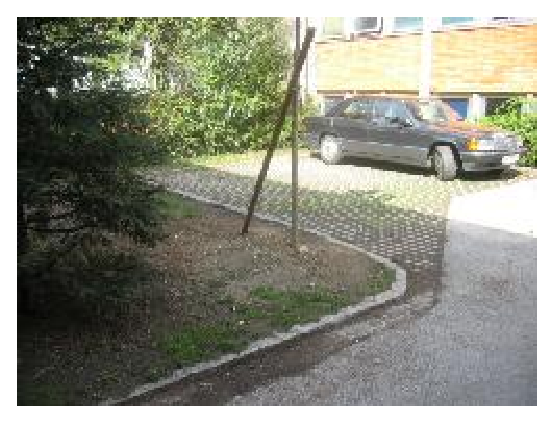
\includegraphics{car}
  \quad
  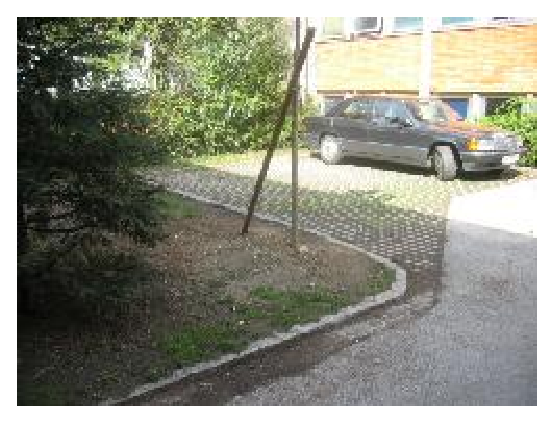
\includegraphics[clip=true,viewport=4.5cm 3.0cm 9cm 6cm]{car}%
\end{figure}
\vfill


%%%%%%%%%%%%%%%%%%%%%%%%%%%%%%%%%%%%%%%%%%%%%%%%%%%%%%%%%%%%%%%%%%%%%%%%%%%%%%%%
\NewPage\headline{\LaTeX \ Tricks: Phantom vs. Itemize}
\vfill
Phantom: \\
Das ist die erste Zeile\\
\phantom{Das ist die erste Zeile} das ist die zweite zeile\\
\phantom{Das ist die erste Zeile das ist die zweite zeile} und die dritte
\vfill
Itemize:\\
\begin{itemize}
  \setlength{\itemsep}{3ex}
  \setlength{\leftmargini}{5em}   
  \setlength{\leftmarginii}{10em}  
  \setlength{\leftmarginiii}{-15em}
\item Das ist die erste Zeile
  \begin{itemize}
  \item das ist die zweite zeile das ist die zweite zeile das ist die zweite zeile das ist die zweite zeile das ist die zweite zeile das ist die zweite zeile
    \begin{itemize}
    \item und die dritte
    \end{itemize}
  \end{itemize}
\end{itemize}
\vfill

%%%%%%%%%%%%%%%%%%%%%%%%%%%%%%%%%%%%%%%%%%%%%%%%%%%%%%%%%%%%%%%%%%%%%%%%%%%%%%%%
\NewPage\headline{\LaTeX \ Tricks: Description}
\vfill
\begin{description}
  \setlength{\itemsep}{3ex}
  \setlength{\leftmargini}{-5em}   
  \setlength{\leftmarginii}{-5em}  
  \setlength{\leftmarginiii}{-5em}
\item[Das ist die erste Zeile] hier geht das nicht das ist die erste
  zeile hier geht das nicht das ist die erste zeile hier geht das
  nicht das ist die erste zeile hier geht das nicht das ist die erste
  zeile das ist die erste zeile
  \begin{description}
  \item[das ist die zweite zeile] das ist die zweite zeile das ist die
    zweite zeile das ist die zweite zeile das ist die zweite zeile das
    ist die zweite zeile
    \begin{description}
    \item[und die dritte zeile] und die dritte zeile und die dritte
      zeile und die dritte zeile und die dritte zeile und die dritte
      zeile und die dritte zeile
    \end{description}
  \end{description}
\end{description}
\vfill

%%%%%%%%%%%%%%%%%%%%%%%%%%%%%%%%%%%%%%%%%%%%%%%%%%%%%%%%%%%%%%%%%%%%%%%%%%%%%%%%
\NewPage\headline{\LaTeX \ Tricks: Embedded Fonts}
\vfill
converts \texttt{foo.pdf}, a file \textcolor{red}{w/o} embedded fonts, into \texttt{foo2.pdf}, a file \textcolor{green}{w/} embedded fonts (\eg for IEEE PDF eXpress):
\begin{itemize}
\item \texttt{gs -sDEVICE=pdfwrite -dPDFSETTINGS=/prepress -dNOPAUSE -q \\ -dBATCH -sOutputFile=foo2.pdf foo.pdf}
\end{itemize}
\vfill 
\alert{There is a bug in in ESP Ghostscript 8.15.x} that may produce a
``drawing error'' in Acroread7.0 but not in xpdf. The newest subversion revision
from January 2006 or e.g\ AFPL Ghostscript 8.53 fixes this problem.

This can cause also ``drawing error'' problems in Acroread7.0 when you use
\texttt{convert} to convert \eg a JPEG/PNG image into an EPS image.
\vfill

%%%%%%%%%%%%%%%%%%%%%%%%%%%%%%%%%%%%%%%%%%%%%%%%%%%%%%%%%%%%%%%%%%%%%%%%%%%%%%%%
\NewPage\headline{\LaTeX \ Tricks: \texttt{write18} Hacks}
\vfill
\begin{verbatim}
\makeatletter
\begingroup
\catcode`\%12\relax
\let\\\relax
\edef\doshell{
date '+%d.%m.%Y %r' |
      awk '{print "\\newcommand*{\\datum}{" $1 "\\xspace}";
            print "\\newcommand*{\\zeit}{" $2 "\\xspace}"
          }' > date.tex
}
\immediate\write18{\doshell}
\endgroup
\makeatother
\newcommand*{\datum}{15.02.2008\xspace}
\newcommand*{\zeit}{11:35:46\xspace}

\end{verbatim}
%%%
\ifpdf
\makeatletter
\begingroup
\catcode`\%12\relax
\let\\\relax
\edef\doshell{
date '+%d.%m.%Y %r' |
      awk '{print "\\newcommand*{\\datum}{" $1 "\\xspace}";
            print "\\newcommand*{\\zeit}{" $2 "\\xspace}"
          }' > date.tex
}
\immediate\write18{\doshell}
\endgroup
\makeatother
\newcommand*{\datum}{15.02.2008\xspace}
\newcommand*{\zeit}{11:35:46\xspace}

This slide was created the \datum at \zeit.
\else
This example needs to be compiled using \\ \alert{\texttt{pdflatex -shell-escape slides.tex}}
\fi
\vfill

%%%%%%%%%%%%%%%%%%%%%%%%%%%%%%%%%%%%%%%%%%%%%%%%%%%%%%%%%%%%%%%%%%%%%%%%%%%%%%%%
\NewPage\headline{\LaTeX \ Tricks: \texttt{write18} Hacks}
\vfill
\begin{verbatim}
\immediate\write18{% 
 echo $USER $HOME $TMPDIR > variables.tex
}
\end{verbatim}
The user, his home-directory und his scratch-directory:
\begin{verbatim}
dreuw /u/dreuw /tmp/dreuw.20080215

\end{verbatim}
\ifpdf
\immediate\write18{% 
 echo $USER $HOME $TMPDIR > variables.tex
}
\alert{dreuw /u/dreuw /tmp/dreuw.20080215
}
\else
\vfill
This example needs to be compiled using \\ \alert{\texttt{pdflatex -shell-escape slides.tex}}
\fi
\vfill


%%%%%%%%%%%%%%%%%%%%%%%%%%%%%%%%%%%%%%%%%%%%%%%%%%%%%%%%%%%%%%%%%%%%%%%%%%%%%%%%
\NewPage\headline{\LaTeX \ Tricks: Fancy verbatim}
\vfill
\begin{Verbatim}[commandchars=\\\{\}] 
  A \textcolor{red}{red word}  within a verbatim environment. 
\end{Verbatim} 
\vfill
program code can be colored by using the listings package, see dante-faq 7.3.4
\vfill

%%%%%%%%%%%%%%%%%%%%%%%%%%%%%%%%%%%%%%%%%%%%%%%%%%%%%%%%%%%%%%%%%%%%%%%%%%%%%%%%
% requires ps-tricks, see style
%  \NewPage\headline{\LaTeX \ Tricks: Creating Nodes}
%  \centering
%  \vfill
%  You can define \rnode{A}{this} as a target.
%  \vfill
%  And create a link from \rnode{B}{here} pointing to the target.
%  \ncarc[linecolor=blue,arcangle=-5]{->}{B}{A}
%  \vfill


%%%%%%%%%%%%%%%%%%%%%%%%%%%%%%%%%%%%%%%%%%%%%%%%%%%%%%%%%%%%%%%%%%%%%%%%%%%%%%%%
\NewPage\headline{Converting And Printing The Slides}
\hypertarget{sli:converting_printing}
\vfill
\begin{itemize}
\item XEmacs editor:
  \begin{itemize}
  \item change into PDF-mode with \texttt{C-c C-t C-p} if you want to create PDF
    slides, otherwise PS slides will be created
  \item run \LaTeX\ with \texttt{C-c C-c}
  \item run again to open the standard viewer \texttt{xpdf} or \texttt{xdvi}
    depending on the mode, \texttt{C-c File} to create a PS-file
  \end{itemize}
\item Creating PDF or PS slides on the command line:
  \begin{itemize}
  \item type \texttt{pdflatex slides} and \texttt{xpdf slides.pdf} to view the
    result
  \item type \texttt{latex slides}, \texttt{dvips slides}, and \texttt{gv
      slides.ps} to view the result
  \end{itemize}
\item Converting:
  \begin{itemize}
  \item use \texttt{dvipdf slides} to convert the created PS-dvi files into
    PDF-slides
  \item use \texttt{dvips slides} to convert the created PS-dvi files into
    PS-slides
  \end{itemize}
\item Handout Printing:
  \begin{itemize}
  \item PDF-slides
    \begin{itemize}
    \item use the Acrobat Reader to print the slides with printer
      option\\ \texttt{/u/hasan/bin/pp -4sup}
    \item or convert the slides with \texttt{pdfnup --nup 2x2
        slides.pdf} and \\print the generated output
      \texttt{slides-2x2.pdf}
    \end{itemize}
  \item PS-slides: use gv with printer option \texttt{/usr/bin/lpz
      -4slidessea} or try \texttt{/u/hasan/bin/pp -4sup}
  \end{itemize}
\end{itemize}
\vfill

%%%%%%%%%%%%%%%%%%%%%%%%%%%%%%%%%%%%%%%%%%%%%%%%%%%%%%%%%%%%%%%%%%%%%%%%%%%%%%%%
\NewPage\headline{FAQ} 
\begin{block}
  If you encounter problems:
  \begin{itemize}
  \item Look at the examples
  \item search in the WWW,\\ 
    \eg in \url{http://groups.google.de/group/de.comp.text.tex}
  \item a4paper/letter problem on Macintosh:\\ 
    try \texttt{ps2pdf -sPAPERSIZE=a4 slides.ps}
  \item Don't ask us, ask \url{http://www.dante.de/faq/de-tex-faq/}
  \item ask us ...
  \end{itemize}
\end{block}


%%%%%%%%%%%%%%%%%%%%%%%%%%%%%%%%%%%%%%%%%%%%%%%%%%%%%%%%%%%%%%%%%%%%%%%%%%%%%%%%
\FinalPage
%%%
\vfill 
\centerline{\footnotesize PS: This page was generated automatically by calling
\texttt{\textbackslash FinalPage}.} 
\vfill
%%%


%%%%%%%%%%%%%%%%%%%%%%%%%%%%%%%%%%%%%%%%%%%%%%%%%%%%%%%%%%%%%%%%%%%%%%%%%%%%%%%%
\NewPage
%\headline{\refname}
%\renewcommand*{\refname}{}
\bibliographystyle{i6bibliostyle}
\bibliography{slides}

%\clearpage
\appendix
%%%%%%%%%%%%%%%%%%%%%%%%%%%%%%%%%%%%%%%%%%%%%%%%%%%%%%%%%%%%%%%%%%%%%%%%%%%%%%%%
\NewPage\headline{\appendixname: First Slide}
\vfill
\hypertarget{anchorname}{Hyper Target} on the first appendix slide. 
Look at the current page number.
\vfill

%%%%%%%%%%%%%%%%%%%%%%%%%%%%%%%%%%%%%%%%%%%%%%%%%%%%%%%%%%%%%%%%%%%%%%%%%%%%%%%%
\NewPage\headline{\appendixname: Table Data}
\vfill
\hypertarget{table_data}{Table Data} on the second appendix slide.
Look at the current page number.
\vfill

\end{document}
